%----------------------------------------------------------------------
%                        PROJECT DEFINITION
%----------------------------------------------------------------------
\renewcommand{\projnr}{C2}
\renewcommand{\projtitleshort}{Modeling dust coagulation}
\renewcommand{\projauth}{Dullemond, Henning}
%
\setcounter{section}{0}
\noindent{\normalfont\sffamily\Large\bfseries Project \projnr: \projtitleshort}
%
\section{Full title:}
\hspace{1\baselineskip}\\
\centerline{\large ``Modeling dust coagulation on a global scale''}
%\centerline{\large ''}
%
\section{General information}\mbox{}
\subsection{Principle investigators:}
\hspace{-\baselineskip}\\\noindent
%
{\bfseries\itshape Dullemond}, Cornelis P., Dr.\\
BAT Ib, non-tenure\\
Date-of-birth: 11 December 1970, Nationality: Dutch\\
Institute: Max-Planck-Institute for Astronomy Heidelberg\\
Street+Nr: K\"onigstuhl 17\\
PLZ+City: 69117 Heidelberg\\
Tel: +49-6221-528-395\\
Fax: +49-6221-528-246\\
Email: dullemon@mpia.de\\
Private address: A.~Rausch Str. 4, 69124 Heidelberg. Tel: 06221-7290263\\
%
\vspace{1em}\\\noindent
{\bfseries\itshape Henning}, Thomas, Prof.~Dr.\\
C4, tenure\\
Date-of-birth: April 9, 1956, Nationality: German\\
DFG Code number of latest application: He 1935/21-2\\
Institute: Max-Planck-Institute for Astronomy Heidelberg\\
Street+Nr: K\"onigstuhl 17\\
PLZ+City: 69117 Heidelberg\\
Tel: +49-6221-528-200\\
Fax: +49-6221-528-246\\
Email: henning@mpia.de\\
Private address: Philosophenweg 3, 69120 Heidelberg. \\


\subsection{Co-investigators within this Forschergruppe:}
\begin{coilist}
\item J.~Blum (IGEP, TU Braunschweig)
\item G.~Wurm (M\"unster)
\item S.~Wolf (MPIA Heidelberg)
%\item K.~Kornet (DFG Emmy Noether group at the MPIA)
%\item F.~Brauer (MPIA Heidelberg)
\end{coilist}


\section{Summary (Zusammenfassung)}
\subsubsection{Summary:} 
We will develop a global model for coagulation and fragmentation of
aggregates and dusty bodies in an evolving protoplanetary disk. Within the
Forschergruppe this project will play the role of connecting the various
projects of the Forschergruppe to each other and put them into a
comprehensive context. We will investigate how the different outcomes of
aggregate collisions (depending on aggregate binding energy, porosity, ice
mantles, and processes such as sintering and eutectic melting) affect the
evolution of the particle size distribution throughout the disk.
%, and how
%particular chemical alterations of the grains get incorporated in aggregates
%through coagulation.  
The ultimate aim is to provide a unified picture of
the process of growth from sub-micron sized particles to kilometer sized
planetesimals based for a large part on the results from the Forschergruppe.

\subsubsection{Zusammenfassung:} 
In diesem Projekt planen wir, ein globales Modell f\"ur die Koagulation und
Fragmentation von Aggregaten und Staubteilchen in einer sich entwickelnden
protoplanetaren Scheibe zu konstruieren.  Innerhalb der Forschergruppe soll
das Projekt die Ergebnisse aus verschiedenen anderen Projekten zu einem
Gesamtzusammenhang zusammen\-f\"ugen. Wir werden untersuchen, wie die
unterschiedlichen Resultate von Teilchenkollisionen die Gesamtentwicklung
der Gr\"o{\ss}enverteilung der Teilchen beeinflussen (in Abh\"angigkeit von
der Bindungsenergie, Porosit\"at, Eism\"antel und Prozessen wie Sintern
und eutektisches Schmelzen).
%, und wie sich eine spezielle chemische
%Ver\"anderung der Staubk\"orner in den Aggregaten aufgrund von Koagulation
%widerspiegelt.
Das ultimative Ziel des Projekts ist die Erstellung eines Gesamtbildes des
Wachstumsprozesses der fr\"uhen Planetenentstehung von sub-mikron gro{\ss}en
Teilchen bis hin zu km-gro{\ss}en Planetesimalen, welches zu einem
gro{\ss}en Teil auf den in dieser Forschergruppe erzielten Ergebnissen
basieren wird.

\section{State of the art (Stand der Forschung)}
\subsection{Overview}
Planetary systems form from the dusty gaseous disks surrounding most young
low mass stars. But in spite of several decades of research it remains an
open issue how this happens. The two main competing scenarios are (a) that
planets form almost instantly by gravitational fragmentation of the gaseous
disk in its very early stages (Kuiper \cit{1951}; Boss
\cit{1997}, \cit{2006}), and (b) that planets form by a lengthy aggregation
and coalescence process, starting from sub-micron sized dust particles, via
multi-km sized `planetesimals', to full-grown planets (Safronov \cit{1969};
Lissauer \cit{1993}; Nakasawa et al.~\cit{2006}). While gravitational
fragmentation may indeed play an important role in the formation of Gas
Giant Planets, there is no doubt that processes like aggregation and
coalescence have taken place in our solar system, which is most clearly
demonstrated by the existence of chondritic meteorites. And for the inner
rocky planets of our solar system there is mounting evidence that
agglomeration of planetesimals and subsequent run-away and oligarchic growth
stands at the basis of their formation (Nakasawa et al.~\cit{2006}). The
objective of this project, and indeed of the entire Forschergruppe, is to
gain a better understanding of the critical first step in this growth
process: the growth from sub-micron dust particles to multi-km sized
planetesimals. We will not only build models, but also compare to
observations (mainly through project \projwolf{}).
A number of reviews give overviews of the current status
of this field (e.g.~Beckwith, Henning \& Nakagawa \cit{2000}; Dominik et
al.~\cit{2006}).

In the stage of growth from dust to kilometer sized objects gravitational
interactions between bodies play only a minor role in the growth
process. Dust grains hit and stick due to relative velocities produced by
their interaction with the gas in the disk.  Vertical sedimentation
(Safronov \cit{1969}) and radial drift (Whipple \cit{1972}) of the dust
causes particles of different sizes to acquire different velocities, and
thus cause preferentially different-size particles to collide and form
bigger aggregates. Turbulence stirs up particles of all sizes and may cause
both equal-sized particles and unequal sized particles to collide and stick
(Mizuno, Markiewicz \& V\"olk \cit{1988}). Depending on the magnitude of the
relative velocities, such collisions can lead to sticking, compaction,
fragmentation, cratering, etc. This is the topic of the studies of
block \blockimpact{} of this Forschergruppe. 
%Exactly which of these outcomes happen,
%depends on the composition and structure of the aggregates, their relative
%velocities, charge etc.\ (see block \blockimpact{} of this Forschergruppe
%proposal). 
But how these outcomes affect the distribution of particles in the
disk is the topic of the present project.

Apart from being the source of the relative velocities required for
aggregation, the processes of sedimentation, radial drift and turbulent
mixing also transport particles throughout the disk. This means that
particles that undergo growth and/or chemical/thermal processing at one
location in the disk can move to another location in the disk and affect the
growth there (Cuzzi, Davis \& Dobrovolskis \cit{2003}; Gail et
al.~\cit{2001}). The process of growth and fragmentation at different
locations in the disk are therefore coupled. An example of this is the
combined sedimentation and growth by a particle sweeping up smaller
particles on its way down to the midplane (Safronov \cit{1969}).  This can
be an effective mode of growth which is very similar to the production of
warm rain on Earth (see e.g.~Kostinski \& Shaw \cit{2005}; Riemer \& Wexler
\cit{2005}). But while the problem of the production of warm rain in the
Earth's atmosphere is that the triggering mechanism is slow, the triggering
of such `rain showers' in protoplanetary disks is extremely fast compared to
the typical life time of such disks (Dullemond \& Dominik \cit{2005}).

Thanks to theoretical models and dedicated laboratory experiments a lot is
now known about how all of these processes work (see e.g.~review by Dominik
et al.~\cit{2006}). However, many fundamental problems remain unsolved (see
below), and the solutions may well lie in the synthesis of all these
processes acting together and influencing each other.

\subsection{Coagulation/aggregation models}
The combined problem of growth and large scale motion of particles in a disk
is a complex one. In the light of the enormous number of particles involved
($\gtrsim 10^{30}$), the use of particle size distribution functions cannot be
avoided. This leads to a complex set of integro-differential equations. In
its simplest form, and without aggregate fragmentation, it can be written as: 
\begin{equation}\label{eq-coag}
\begin{split}
\frac{\partial n(\vec x,m)}{\partial t} &= 
\int_{m_\mathrm{min}}^{m/2}
K(\vec x,m',m-m')\,n(\vec x,m')\,n(\vec x,m-m')\,dm'  \\
& -\int_{m_\mathrm{min}}^{m_{\mathrm{max}}}
K(\vec x,m',m)\,n(\vec x,m')\,n(\vec x,m)\,dm'\\
& - \nabla \cdot [n(\vec x,m) \vec v(\vec x,m)] 
+ \nabla \cdot \left[D(\vec x,m)\rho_g(\vec x)
\nabla \left( \frac{n(\vec x,m)}{\rho_g(\vec x)} \right)\right] ,
\end{split}
\end{equation}
where $m$ is the mass of the particle, $\vec x$ is spatial position, $n(\vec
x,m)$ is the particle distribution function, $\vec v(\vec x)$ is the drift
velocity relative to the gas (assumed static in this simple form of the
equations), $D(\vec x,m)$ the turbulent diffusion coefficient of the
particles within the gas, and $K(\vec x,m_1,m_2)$ the coagulation kernel for
growth, which incorporates all the physics and details of the individual
collisions (i.e.~which of the various possible collision outcomes mentioned
above will happen, and how).  The first part of the right-hand-side of
Eq.(\ref{eq-coag}), i.e.~the terms with the aggregation integrals,
represents the continuous form of the {\em Smoluchowski equation}
(Smoluchowski \cit{1916}). If fragmentation is included, various other terms
need to be added to this equation (see e.g.~Th\'ebault et al.\
\cit{2003}). The second part of Eq.(\ref{eq-coag}) represent the advection
and mixing terms. These terms depend of course also on systematic motion of
the gas, which is not included in this simplified form of the equation.

First models of grain growth based on Eq.(\ref{eq-coag}) and its
generalizations were made in the eighties (Weidenschilling \cit{1980},
\cit{1984}; Nakagawa, Nakazawa \& Hayashi~\cit{1981}), but computational
cost vastly exceeded computer capabilities at that time, resulting in
somewhat crude models. Moreover, the coagulation kernel, which plays a
decisive role in the outcome of the evolution of the dust population, was
poorly known. Currently much more is known about the
coagulation/fragmentation kernel thanks to laboratory experiments (see
review by Dominik et al.~\cit{2006} and literature overview in Projects
\projblum{} and \projwurm{}) and numerical modeling (Dominik \& Tielens
\cit{1997}; Benz \& Asphaug~\cit{1994}; Sirono \& Greenberg~\cit{2000}),
although there is still a long path ahead before a reasonable complete
picture of the coagulation/fragmentation kernel is assembled.

More recent models based on these equations are: Mizuno, Markiewicz \&
V\"olk (\cit{1988}) on turbulent coagulation in disks; Weidenschilling
(\cit{1997}) on the formation of comets in the Kuiper belt; Schmitt, Henning
\& Mucha (\cit{1997}) on the feedback of coagulation on the disk evolution;
Suttner \& Yorke (\cit{2001}) on dust coagulation in the formation stages of
the disk; Dullemond \& Dominik (\cit{2005}) and Tanaka, Himeno \& Ida
(\cit{2005}) on the effect of coagulation on disk spectra, and Nomura \&
Nakagawa (\cit{2006}) on the growth of grains and the formation of a
thin unstable midplane layer.

The above papers have developed and used various algorithms for solving the
coagulation equation. A systematic study of potential numerical artifacts
from coagulation calculations was made by Ohtsuki, Nakagawa \& Nakazawa
(\cit{1990}). The problem of coagulation also plays an important role in
industry and meteorology, and in that context there is also a large volume
of literature on numerical methods of solving these equations (see
e.g.~Kraft \cit{2005} for a review).

Although models based on Eq.(\ref{eq-coag}) are necessary and useful for
studying the problem of planetesimal formation, we are very aware of the
various limitations of Eq.(\ref{eq-coag}): the simplicity of the diffusion
approximation for turbulence, the breakdown of the continuous particle
distribution approximation for run-away growth and various other problems.


\subsection{Main open questions}
Models based on Eq.~(\ref{eq-coag}) and its generalizations, require the
specification of a significant volume of input physics. The main piece of
input physics is the coagulation kernel $K(\vec x,m_1,m_2)$ and its
generalizations. Laboratory data (see projects
\projblum{}, \projwurm{} and \projblumtrie{}) as well as numerical
simulations of collisions (see project \projkley{}) give values of sticking
coefficients and fragmentation distributions for a (limited) discrete set of
initial collision conditions and initial aggregate structures. So far the
coverage of this parameter space is far from complete. High velocity impacts
have only recently been modeled (Wurm, Paraskov \& Krauss~\cit{2005}), and
the exploration of impacts of porous projectiles onto larger porous targets
have also only recently been started (Langkowski \& Blum \cit{in
prep.}). Many effects that might influence the outcome of collisions (and
are therefore part of the coagulation kernel) have as yet been
unexplored. Moreover, as part of the coagulation kernel the relative
velocities induced by turbulence (e.g.~V\"olk et al.~\cit{1980};
Weidenschilling \cit{1984}) and drift are still under debate (see project
\projklahr{}). The role of turbulence for diffusive transport, which sets
the coefficient $D(\vec x,m)$ in Eq.~(\ref{eq-coag}), is also still debated
(Johansen et al.~\cit{2005}; Carbillado, Stone \& Pringle
\cit{2005}). Uncertainties in $D(\vec x,m)$ are up to a factor of 10, which
can have major influence on the transport processes (Dullemond, Apai \&
Walch \cit{2006a}).  .

One of the main problems for aggregate growth is the `meter-size
barrier'. At 1 AU distance from the star particles of about 1 m in size have
a radial drift velocity that is so large that they drift inward to the
evaporation radius faster than they can continue to grow (Whipple
\cit{1972}; Weidenschilling \cit{1977}). Moreover, even if they do not
drift, their relative velocities are so large, that any collisions will
fragment them upon a collision (e.g.~Blum \& Wurm \cit{2000}). Various
scenarios have been suggested to `jump over' this meter-size
barrier. Goldreich \& Ward (\cit{1973}) suggested that in the absence of
turbulence the dust sediments to a very thin midplane layer which eventually
becomes gravitationally unstable and fragments into clumps which form
planetesimals. But Weidenschilling (\cit{1977}), Cuzzi, Dobrovolskis \&
Champney (\cit{1993}) and Johansen, Henning \& Klahr (\cit{2006}) have shown
that Kelvin-Helmholtz instabilities are triggered in such a layer, causing
turbulence which puffs up the layer before it becomes thin enough for
gravitational collapse. Moreover, even if such a gravitational instability
sets in, it is unclear if the collisional dissipation of kinetic
`temperature' of the swarm of particles is efficient enough for these
instabilities to produce planetesimals (e.g.~Weidenschilling
\cit{1997}). Recently, however, Youdin \& Shu (\cit{2002}) have re-examined
the problem and argued that an enhancement of solid material caused by
radial drift of particles from larger radii may help overcome these problems
(see, however, the discussion in Dominik et al.~\cit{2006}). These
scenarios, however, require zero intrinsic turbulence (i.e.~no
magneto-rotationally driven turbulence, see Balbus \& Hawley
\cit{1991}; Semenov et al.~\cit{2004}; Ilgner \& Nelson
\cit{2006}). But the observed geometric shape of protoplanetary disks
(e.g.~Burrows et al.~\cit{1996}; Throop et al.~\cit{2001}) clearly shows
that a significant amount of turbulence is present to keep the small grains
suspended in the gas. So recent new ideas to jump over the meter-size
barrier include particle concentration in vortices (e.g.~Barge \& Sommeria
\cit{1995}; Klahr \& Henning \cit{1997}), in turbulent eddies (Johansen et
al.~\cit{2006}), and in spiral waves (Rice et al.\ \cit{2004}).  Another
scenario invokes the concept of 'luck': the very few objects that happen to
survive the meter-size barrier (approx.\ 1:$10^9$) continue to grow by
sweep-up of smaller particles and eventually become planetesimals
(Weidenschilling \cit{1997}; Dullemond \& Dominik \cit{2005}). In all of the
above scenarios turbulence clearly plays a decisive role, but it is one of
the main unknowns what precisely this role is.

Once a body manages to cross the meter-size barrier, the high relative
velocities between multi-meter sized bodies and very much smaller particles
($\lesssim$ 1 cm) also poses a problem. It is, as yet, not fully clarified
whether large numbers of impacts of smaller particles on bigger objects will
cause them to grow or erode. This is, in fact, the topic of several projects
of the Forschergruppe (block B). 
%
%A large volume of research is being done at
%present to clarify this (see literature overviews in projects \projblum{}
%and \projwurm{}), but it is as yet 
%
It is as yet also unclear how these results work out on the overall size
distribution of the aggregates. It is not well known, for instance, how the
debris from such impacts affect the size distribution of the particles, how
the average structure of the aggregates/bodies changes with time
(compaction, fracturing etc), what the dominant collision partners are
(which size particle collides preferentially with which other size), and
what the main mode of growth is (ordered growth, sweep-up growth, etc.). In
addition to this, thermal processing of the grains may affect the sticking
properties of the particles (see project \projblumtrie{}), and may provide
important trace-markers for the transport of particles (see project
\projtscharn{}) which is also important to explain the mineralogical
composition of meteorites and comets and of protoplanetary disks. Charge
exchange between particles upon collisions is known in the Earth's
atmosphere to play an important role. A similar phenomenon is thought also
to play a role in disks, and might affect the sticking probability of
particles, which is still unexplored (see project \projblum{}). 
%The systematic charging of these
%particles, the movement of these charged particles throughout the disk, as
%well as the effect that the increased sticking probability has on the size
%distribution are also unexplored as yet.

Another thing which is not yet fully explored is the effect of the disk
formation process and the disk's viscous evolution on the grain size
distribution. Some work along these lines has been published by Suttner \&
Yorke (\cit{2001}) and Schmitt, Henning \& Mucha (\cit{1997}), but the time
spans of these simulations was limited.

Finally, since the recent surge of observational data from protoplanetary
disks and their dust content, a number of major new questions have arisen.
First of all, the observations in the infrared only trace the surface 
layers of the disk. The question is what the information about grain sizes
in the surface layers tells about the grain population at the midplane.
Second: observations only trace grains with sizes $\lesssim$ 1 cm, so the
question is: what does this tell about the particles $\gtrsim$ 1 cm? A third
question is: what is the cause for the observed grain sizes, and which clues
does this give to the overall aggregation process?

The present project will address many of these issues with a model of
coagulation, with input physics from projects B1, B2, B3, B4, A2 and C1,
and with output to projects D1 and D2 for comparison to measurements
of our own solar system and protoplanetary disks.

\section{Preliminary work (Eigene Vorarbeiten)}\label{sec-prelim}
\subsection{General earlier own work}
An important basis upon which coagulation models are built is a model of the
structure and evolution of the protoplanetary disk. Early models of the
disk structure were made (among others) by Bell, Cassen, Klahr \&
Henning~(\cit{1997}), Dullemond, Dominik \& Natta (\cit{2001}), Dullemond,
van Zadelhoff \& Natta (\cit{2002}) and Dullemond \& Natta
(\cit{2003a,2003b}). These were 1+1D models, i.e.\ nearly independent 1-D
vertical structure models glued together to form a 1+1D disk structure. An
improvement of that, based on 2-D radiative transfer, was developed by
Dullemond (\cit{2002}) and refined by Dullemond \& Dominik
(\cit{2004}). These models (as well as similar models from competitors) are
able to explain various observational aspects of protoplanetary disks,
including their dust emission features, the spectral energy distribution
shape, disk images etc.~(see e.g~Dullemond et al.~\cit{2006c} for a review on
disk structure models). 

Inspired by earlier work of Nakamoto \& Nakagawa (\cit{1994}) and of Hueso
\& Guillot (\cit{2005}), models were made for the time-dependent formation
and viscous evolution of protoplanetary disks (Dullemond, Apai \& Walch
\cit{2006a}). This work shows that crystalline silicates observed in such
disks may originate from the very early stages of disk formation. The same
models were also shown to be able to explain a hitherto unexplained observed
trend of accretion rate $\dot M$ with stellar mass $M_{*}$ in the Taurus and
$\rho$-Ophiuchus clusters (Dullemond, Natta \& Testi \cit{2006b}).

A crucial part of the coagulation modeling is the modeling of the motion of
particles. Schr\"apler \& Henning (\cit{2004}) studied in
detail the effect of turbulence on the sedimentation of grains to the
midplane of the disk. The effect of sedimentation on the spectra of disks
was studied by Dullemond \& Dominik (\cit{2004}).

Models of aggregation on the microscopic level were made by Kempf, Pfalzner
\& Henning (\cit{1999}) and by Ossenkopf \& Henning (\cit{1994}), which can
serve as input to the coagulation kernel. Coagulation models (based on
equations like Eq.~\ref{eq-coag}) for the very early stages of disk
evolution were presented by Schmitt, Henning \& Mucha (\cit{1997}), who also
study the back-reaction of grain growth on disk evolution. The first
comparison of a full dust coagulation model to observed spectra of
protoplanetary disks was published by Dullemond \& Dominik (\cit{2005}).
They conclude that coagulation without fragmentation is too effective in
removing small grains from the disk to be consistent with observations of
protoplanetary disks. This paper also discussed and studied a scenario of
survival of bodies through the meter-size barrier, in which a few
`lucky ones' survive the meter size barrier without a major collision,
and once they are beyond the dangerous regime, they continue to grow
by sweeping up dust.

In addition to these, the PIs have been involved in many projects which are
related to this topic: (a) Observations of spectra of dust in protoplanetary
disks (e.g.~Kessler-Silacci et al.~\cit{2006}; Apai et al.~\cit{2005};
Rodmann et al.~\cit{2006}; van Boekel et al.~\cit{2004}), (b) Radiative
transfer modeling of observations of disks (e.g.~Wolf, Henning \& Stecklum
\cit{1999}; Pontoppidan et al.~\cit{2005}), (c) Calculation of optical
properties of grains (e.g.~Henning et al.~\cit{1999}), (d) Hydrodynamics of
dusty turbulent gases (e.g.~Johansen, Klahr \& Henning \cit{2006}).



\subsubsection{Special preparations for the proposed project}\label{sec-special-prep}
The main tool for the proposed project is the aggregation/fragmentation
computer program. Currently this coagulation code is being further developed
by a PhD student (Brauer) and the PI (Dullemond) in the following three
ways, which are relevant for the proposed project:
\begin{enumerate}
\item A detailed sedimentation/mixing model is being developed for the
vertical structure of the dust of a given mass $m$. Solved are its density
structure $n(z,m)$ for a given value of $\sigma(m)\equiv \int_0^\infty
n(z,m)dz$, as well as the radial and azimuthal velocities of the gas and the
dust ($v_{g,r}(z)$, $v_{g,\phi}(z)$, $v_{d,r}(z,m)$,
$v_{d,\phi}(z,m)$). This models includes collective effects with gas-dust
friction (see Nakagawa, Sekiya \& Hayashi \cit{1986}), vertical viscosity in
both $r$ and $\phi$ velocity components (Takeuchi \& Lin \cit{2002}), and
covers both {\em given} turbulence (Dubrulle et al.~\cit{1995}) and/or {\em
self-induced} turbulence (Weidenschilling \cit{2006}). We plan to submit
this paper in the summer of 2006.
\item An implicit method of numerical solution for the combined coagulation
and fragmentation is being developed. This code will contain the numerical
algorithms, but contains only a basic coagulation/fragmentation kernel.
First version of the code is currently in the testing phase. A useable
version is expected to be ready by the end of 2006 at the latest.
\item Combining the vertical model (point 1) with the
coagulation/fragmentation code (point 2). Putting this on a time-dependent
disk formation and evolution model (Dullemond, Apai \& Walch \cit{2006a}, with
expertise input from project \projtscharn{}). 
% Include radial drift and
% radial mixing by integrating the 1-D {\em vertical} models at each radius to
% obtain vertically-integrated quantities as a function of $r$ that can be
% inserted in a 1-D {\em radial} model (see Takeuchi \& Lin \cit{2002} for an
% example of such a radial model). After one time step of disk evolution,
% radial drift and mixing, the 1-D vertical model is used to expand the model
% back to 1-D {\em vertical} models at each radius, where the coagulation can
% be computed again. 
This work is at present in the planning phase, and will likely be developed
in collaboration with the PhD student of the present proposal (see work
plan).
\end{enumerate}
Should the implicit integration turn out not to work as expected, we will
stick with our current explicit integration method and will employ parallel
computing power (which is available at the MPIA): one processor for each
vertical 1-D slab, requiring roughly 1 week for one run.

% By the start of the Forschergruppe, or at the latest after the first 6
% months of the Forschergruppe, development 1 and 2 will be ready and useable
% for the the project we propose here. At the latest during the next year (up
% to the middle of the 2nd year of the Forschergruppe) the development 3 is
% planned to be ready, but this is less essential for the project proposed
% here. Should the implicit integration turn out not to work as expected, we
% will stick with our current explicit integration method and will employ
% parallel computing power (which is available at the MPIA): one processor for
% each vertical 1-D slab, requiring roughly 1 week for one run.  {\em In any
% case, the current PhD student, F.~Brauer, will be able to provide
% substantial help and guidance to the PhD student of this proposal until
% Brauer's expected PhD defense, April 2008}. This will be of importance in
% the light of the challenging nature of the presently proposed project.




%
% Here follows the own refereed publications by the PIs in relation to
% the project proposed here.
%
\ownpubltitle{Own publications related to the Forschergruppe:}
%
% BELOW IS ONLY AN EXAMPLE OF TWO ENTRIES. SEE THE ADDITIONAL FILES 
% SENT TO YOU WITH ALL THE REFERENCES FROM THE VORANTRAG
%
\begin{ownpubl}
\item Acke, B., van den Ancker,  M.E., Dullemond, C.P., van Boekel, R. \&
  Waters, L.B.F.M. Evidence for grain growth in self-shadowed disks
  around Herbig Ae/Be stars (2004) \aap \textbf{422}, 621
\item Apai, D., Pascucci, I., Sterzik, M.F., van der Bliek, N., Bouwman, J.,
  Dullemond, C.P. \& Henning, Th. 
  Grain growth and dust settling in a brown dwarf disk: Gemini/T-ReCS
  observations of CFHT-BD-Tau 4 (2004) \aap \textbf{426}, 53
\item Apai, C.,  Pascucci, I., Bouwman, J., Natta, A., Henning, Th. \&
  Dullemond, C.P. (2005) The onset of planet formation in Brown Dwarf disks
  \sci \textbf{310}, 834
\item Bell, K.R., Cassen, P.M., Klahr, H.H. \& Henning Th. (1997)
  The Structure and Appearance of Protostellar Accretion Disks: Limits on
  Disk Flaring, \apj \textbf{486}, 372
\item Dullemond,~C.~P., Natta, A. \& Testi, L. (2006b) Accretion in
  protoplanetary disks: the imprint of core properties, \apj in press
\item {Dullemond}, C.~P. and {Apai}, D. and {Walch}, S. (2006a)
  Crystalline Silicates as a Probe of Disk Formation History, 
  \apjl \textbf{640}, 67
\item {Dullemond}, C.~P. and {Dominik}, C. (2005) Dust coagulation in
  protoplanetary disks: A rapid depletion of small grains, \aap
  \textbf{434}, 971
\item {Dullemond}, C.~P. and {Dominik}, C. (2004b) The effect of dust
  settling on the appearance of protoplanetary disks, \aap
  \textbf{421}, 1075 
\item {Dullemond}, C.~P. and {Dominik}, C. (2004a) Flaring
  vs. self-shadowed disks: The SEDs of Herbig Ae/Be stars, \aap
  \textbf{417}, 159
\item {Dullemond}, C.~P. and {Natta}, A. (2003b) An analysis of two-layer
  models for circumstellar disks, \aap \textbf{405}, 597
\item {Dullemond}, C.~P. and {Natta}, A. (2003a) The effect of scattering on
  the structure and SED of protoplanetary disks, \aap \textbf{408}, 161
\item {Dullemond}, C.~P. and {van Zadelhoff}, G.~J. and {Natta}, A.
  (2002) Vertical structure models of T Tauri and Herbig Ae/Be disks,
  \aap \textbf{389}, 464 
\item {Dullemond}, C.~P. (2002) The 2-D structure of dusty disks around
  Herbig Ae/Be stars. I.  Models with grey opacities, \aap \textbf{395}, 853
\item {Dullemond}, C.~P., {Dominik}, C. and {Natta}, A. (2001)
  Passive Irradiated Circumstellar Disks with an Inner Hole, \apj
  \textbf{560}, 957
\item Dominik, C., Dullemond, C.P., Waters, L.B.F.M.~\& Walch, S. (2003)
  Understanding the spectra of isolated Herbig stars in the frame of a passive
  disk model, \aap \textbf{398}, 607
\item Henning, Th., Il'In, V.B., Krivova, N.A., Michel, B. \& Voshchinnikov,
  N.V. (1999) WWW Database of optical constants for astronomy, 
  \aaps \textbf{136}, 405
\item Johansen, A., Klahr, H. \& Henning, Th. (2006) Gravoturbulent 
  formation of planets, \apj \textbf{636}, 1121
\item Johansen, A., Henning, Th. and  Klahr, H. (2006) 
  Dust sedimentation and self-sustained Kelvin-Helmholtz turbulence
  in protoplanetary disk mid-planes. 
  I. Radially symmetric simulations. \apj, in press
\item Kempf, S., Pfalzner, S. \& Henning, Th. (1999) N-Particle-Simulations
  of Dust Growth. I. Growth Driven by Brownian Motion, \ica \textbf{141}, 388 
\item Kessler-Silacci, J., Augereau, J.-C., Dullemond, C.P., et al. (2006)
  c2d Spitzer IRS spectra of disks around T Tauri stars. I. Silicate emission
  and grain growth, \apj \textbf{639}, 275
\item Ossenkopf, V. \& Henning, Th. (1994) Dust opacities for protostellar
  cores, \aap \textbf{291}, 943
\item Pascucci, I., Apai, D., Henning, Th.~\& Dullemond, C.~P. (2003) The
  First Detailed Look at a Brown Dwarf Disk, \apjl \textbf{590}, 111
\item Pontoppidan, K. \& Dullemond et al., C.P., (2005) Spitzer spectroscopy
  and 2D modeling of the edge-on disk CRBR 2422.8-3423 \apj \textbf{622}, 463
\item Schr\"apler, R. \& Henning, Th. (2004) Dust Diffusion, Sedimentation,
  and Gravitational Instabilities in Protoplanetary Disks, 
  \apj \textbf{614}, 960
\item Rodmann, J., Henning, Th., Chandler, C.J., Mundy, L.G. \& Wilner, D.J.
  (2006) Large dust particles in disks around T Tauri stars, 
  \aap \textbf{446}, 211
\item Schmitt, W., Henning, Th. \& Mucha, R. (1997) Dust evolution in
  protoplanetary accretion disks, \aap \textbf{325}, 569
\item van Boekel, R., Waters, L.B.F.M., Dominik, C., Bouwman, J., de Koter,
  A., Dullemond, C.P., Paresce, F. (2003) Grain growth in the inner regions of
  Herbig Ae/Be star disks, \aapl \textbf{400}, 21
\item van Boekel, R., Min, M., Leinert, Ch. et al. (2004) The building
  blocks of planets within the `terrestrial' region of protoplanetary disks,
  \nat \textbf{432}, 479
\item van Boekel, R., Waters, L.~B.~F.~M., Dominik, C., Dullemond, C.~P.,
  Tielens, A.~G.~G.~M.~\& de Koter, A. (2004) 
  Spatially and spectrally resolved 10 $\mu$m emission in
  Herbig Ae/Be stars, \aap \textbf{418}, 177
\item Wolf, S., Henning, Th. \& Stecklum (1999) Multi-dimensional
  self-consistent radiative transfer simulations based on the Monte
  Carlo method, \aap \textbf{349}, 839
\end{ownpubl}
%
%
%
%
\section{Goals (Ziele)}
The main objective is to put the various topics of the Forschergruppe into
each other's context, and thereby addressing the main objectives listed in
the `scientific objectives' of the Forschergruppe. More specifically:

%{\bf\LARGE REFORMULATE THE GOALS}
\begin{enumerate}
\item Develop a ``next-generation aggregation model'', which acts as a
unification of various projects within the Forschergruppe:
\begin{enumerate}
\item Construct realistic expressions for the coagulation kernel $K$ 
(including fragmentation, charge, porosity / fractal dimension etc.), the
turbulent particle diffusion coefficient $D$ and the average drift velocity
$v$ that go into Eq.~(\ref{eq-coag}). This will be based on the input from
various projects within the Forschergruppe (\projblum{}, \projwurm{},
\projblumtrie{}, \projkley{}, \projklahr{}, \projtscharn) and on earlier
laboratory results and computer simulations of collisions.
\item Perform simulations to discover the ways by which the various physical
processes studied by the Forschergruppe affect each other and the overall 
growth of aggregates.
\item Find out what is the relative importance of the various processes 
studied in this Forschergruppe. Which processes dominate where and when?
\item Provide feedback to the above mentioned projects: which new
experiments/simulations are needed to improve the aggregation model, and
which kind of conditions are too rare to be worthwhile to study in the
laboratory / computer simulation?
\end{enumerate}
%Special focus will be on implementing and following the effect of 
%material properties (porosity, mineralogy, ice-coatings) and grain charge 
%on the overal growth and evolution of particle distribution function.
\item Apply the code to address the following issues:
\begin{enumerate}
\item What are the time scales for the formation of planetesimals at
various positions in the disk, or for
the formation of smaller sized objects that may rapidly (by gravitational
instability) assemble to form planetesimals?
\item What is the spatial distribution of particles of various sizes, and
how does this change over time, and why?
%\item How do the various size particles influence each other? What does
%the population of small particles and their disappearance over time
%tell about the larger paticles in the disk?
%\item What are the expected compositions of asteroids and comets (having 
%incorporated materials transported to the final assembly site by various
%mechanisms)?
%\item Can large-scale charge separation take place in the disk?
\item What is the main mode of growth in various stages of the disk
life time (sweep-up, run-away, ordered)?
\item How does grain growth in the very earliest disk phases ($t\lesssim
10^5$ years), where the disk is still being formed through infalling matter
from the parent cloud, affect the grain population in the later stages? How
does the time-dependent viscous evolution of the disk affect the growth?
\item How does gradual gas removal, through e.g.~photoevaporation in the
end stages of the disk ($t\gtrsim 3\times 10^6$ years), affect the growth /
fragmentation?
\item Can big bodies like planetesimals and cometesimals form in turbulent 
disks? Observations show that disks must be at least somewhat turbulent, but
certain models rely on the absence of systematic (non-self-induced)
turbulence (e.g.~Weidenschilling \cit{1997}).
\end{enumerate}
\item In close collaboration with project \projwolf{} we will confront our
models with observations of protoplanetary disks. Two examples of such
comparisons are:
\begin{enumerate}
\item Pure grain growth would deplete the small grains much faster than is
observed (Dullemond \& Dominik~\cit{2005}, and references therein). Can
fragmentation of aggregates replenish the small dust grain population for a
sufficient amount of time?  And on which time scales do the small dust
grains eventually disappear nonetheless? Is this consistent with observed
disk dispersal rates (Haisch et al.~\cit{2001}; Carpenter~\cit{2005}), and
the formation of gaps (e.g.~Forrest et al.~\cit{2004})? And how does this
relate to the observed non-correlation between grain size-indicators and
stellar age? \label{dulgoal-smallgrains}
%\item What is the cause of the observed correlation between grain growth and
%crystallinity of grains in protoplanetary disks (van Boekel et al.~##{vBo05})?
%Can observations of crystallinity be used as a proxy of grain growth?
%\label{dulgoal-crystgrowth}
\item Recent centimeter observations of TW Hydra indicate that the large
grain population ($\sim$ 2.5 cm) is dominated by a narrow size distribution
peak (Wilner et al.~\cit{2005}). Modeling this may give clues to the binding
strength of the dust aggregates.\label{dulgoal-willner}
\end{enumerate}
In this collaboration we will also attempt to:
\begin{enumerate}
\item identify ways in which the study of observable dust grains ($a\lesssim
1$ mm) in protoplanetary disks by infrared and (sub-)millimeter telescopes
provide clues to the {\em unobservable} process of growth from $a\sim 1$ mm
to multi-kilometer planetesimals.\label{dulgoal-linkobs}
\item identify ways in which the observable grains in the {\em surface
layers} of the disk provide clues to the unobservable grains {\em deeply
embedded within the disk}.
\end{enumerate}
\end{enumerate}



\section{Work schedule (Arbeitsprogramm)}
\subsection{Methods}
\subsubsection{Available tool set}
As a basis of our project we have the following modeling tools available:
\begin{itemize}
\item Detailed disk stationary structure models in 1+1D and 2-D from 
the PI (Dullemond \cit{2002}; Dullemond et al.~\cit{2002}; Dullemond
\& Natta \cit{2003a,2003b}; Dullemond \& Dominik \cit{2004a}). A close
collaboration with the team of project A2 will also allow exchange of
expertise and algorithms on this point.
\item Time-dependent disk formation and viscous evolution models with a simple
recipe of radial mixing (Dullemond, Apai \& Walch \cit{2006}; Dullemond,
Natta \& Testi \cit{2006}).
\item A 1+1D sedimentation/aggregation/fragmentation code (Dullemond \& 
Dominik~\cit{2004b,2005}; Brauer et al.~in prep, see Section
\ref{sec-special-prep}) for modeling grain coagulation, fragmentation,
sedimentation and radial drift with size distribution functions (see Section
\ref{sec-prelim}). Two coagulation algorithms are implemented: 
the algorithm developed by Dullemond \& Dominik (\cit{2005}) as well as 
that of Kovetz \& Olund (\cit{1969}, often called the `Podolak
algorithm'). An example of the grain size distributions as a function
of time is shown in Fig.~\ref{fig-lucky}. Also on this point, a
collaboration with the project A2 will allow exchange of expertise: project
A2, while focusing on the chemistry, also needs some knowledge of grain
growth, while project C2 (this project), focusing on growth, also needs some
input on the composition of the grains.
\end{itemize}

\begin{figure}[t]
\centerline{\includegraphics[width=10cm]{c2fig1.eps}}
\caption{\label{fig-lucky}The time-dependent size distribution at the 
midplane of a disk at $r=$ 1 AU for an aggregation problem with a simple
form of fragmentation included, calculated using our methods. From
light-grey to dark grey the times are $10^{0,1,2,3,4,5}$ year respectively.
Around $t=10^4$ yr a semi-steady state sets in up to cm size. In this steady
state there is a balance between growth and destruction of aggregates. At
larger aggregate sizes there are a few `lucky ones' (about 1:10$^9$) who
have survived the fragmentation barrier (in this particular set of
parameters and input physics located at $\sim$ 10 cm) and continue to grow
by sweep up of particles from the semi-steady-state reservoir of $\lesssim$
1 cm particles. This calculation does not yet include any details of
erosion, cratering, radial drift etc.}
\end{figure}



\subsubsection{Building a realistic coagulation kernel}
For pure coagulation/aggregation without fragmentation, and for given
(known) aggregate properties as a function of mass $m$, the kernel can be
written as:
\begin{equation}\label{eq-kernel-1}
K(\vec x, m_1, m_2) = \int_0^\infty \eta(m_1,m_2,\Delta v)\;
\sigma(m_1,m_2)\; \Delta v\; P(\Delta v;\vec x,m_1,m_2)\; d \Delta v
\end{equation}
where $\sigma(m_1,m_2)$ is the collision cross-section, $\eta(m_1,m_2,\Delta
v)$ the sticking probability for particles of masses $m_1$ and $m_2$
colliding with a velocity $\Delta v$ (averaged over all possible impact
parameters), and $P(\Delta v;\vec x,m_1,m_2)$ the probability function for
the relative velocities between these particles.  Ideally one should perform
lab experiments and collision model calculations (input from projects \projblum{},
\projwurm{}, \projblumtrie{}, \projkley{}) for all combinations of $m_1$,
$m_2$ and $\Delta v$, on a fine grid in all three parameter dimensions.
Obtaining each of these values requires an averaging over all possible
impact parameters. This implies a fine-spaced scanning of a 4-D parameter
space, which is in practice impossible. The best one can obtain is a limit
set of points within this $(m_1,m_2,\Delta v)$ parameter space. To create a
smooth coagulation kernel from this, three methods can be employed: (1) a
simple semi-analytic model, (2) a simple fitting formula and (3) an
interpolation sub-routine on the measurements.

The laboratory experiments and collision models are only one factor of the
coagulation kernel. An equally important, and equally challenging, factor is
the velocity probability function $P(\Delta v;\vec x,m_1,m_2)$.  Relative
velocities caused by systematic differential drift of particles (be it
sedimentation or radial drift) produce non-disperse velocity distributions:
$P(\Delta v)=\delta(\Delta v-|\vec v_2-\vec v_1|)$. Brownian motion and
turbulence, however, produce random motions and therefore produce a
broadening of the velocity probability function. In particular for
turbulence this velocity distribution function is rather complex. An often
used simplification is to take only average relative velocities into
account. In this case the entire relative velocity probability function
$P(\Delta v)$ becomes a $\delta$-function and Eq.~(\ref{eq-kernel-1})
reduces to:
\begin{equation}\label{eq-kernel-2}
K(\vec x, m_1, m_2) = \eta(m_1,m_2,\langle\Delta v\rangle)\;
\sigma(m_1,m_2)\; \langle\Delta v\rangle
\end{equation}
The value of $\langle\Delta v\rangle$ for particles in turbulent gases have
been calculated numerically by V\"olk (\cit{1980}), Mizuno, Markiewicz \&
V\"olk (\cit{1988}), and analytic fitting formulae were derived by
Weidenschilling (\cit{1984}). But these expressions were derived under
standard assumptions for Kolmogorov turbulence. It remains unverified
whether turbulence driven by Kelvin-Helmholtz instabilities (Weidenschilling
\cit{1977}; Cuzzi et al.~\cit{1993}; Johansen \& Klahr in prep.) and/or by
magneto-rotational instability (Balbus \& Hawley \cit{1991}; Brandenburg et
al.~\cit{1996}) are of the same nature.  Moreover, it remains uncertain
whether this average-$\langle\Delta v\rangle$ approach is valid in the first
place. There are examples from meteorology in which statistical fluctuations
seem to play a major role, like in the formation of warm rain on Earth
(Kostinski \& Shaw \cit{2005}). Project \projklahr{} will play a vital role
at this point. It will provide knowledge of $P(\Delta v;\vec x,m_1,m_2)$
which is the required input here. In collaboration with that project, we
will attempt to develop fitting formulae to summarize the expected complex
functionality of $P(\Delta v;\vec x,m_1,m_2)$. We will also investigate the
importance of the above mentioned statistical fluctuations.
%  If, as hoped,
% Eq.~(\ref{eq-kernel-2}) can be used without too large problems, one of the
% tasks of project \projklahr{}, i.e.\ finding a proper expression of
% $P(\Delta v;\vec x,m_1,m_2)$, can then be reduced to finding an expression of
% $\langle\Delta v\rangle$ as a function of $\vec x$, $m_1$ and $m_2$.

The $\langle\Delta v\rangle$-approach can also introduce another problem:
for a sufficiently wide velocity distribution one could have sticking for
the lower velocity part and shattering for the higher velocity part.
Using a single $\langle\Delta v\rangle$ will ignore this effect. We will
investigate how important this effect is, and if it is important we will 
derive separate expressions for $\langle\Delta v\rangle$ for the
sticking and shattering regime.

In collaboration with project \projklahr{} we will also investigate the
effect of in homogeneities (e.g.~particle trapping) on the coagulation. 
We will develop a simple empirical `model' that describes this effect,
so that it can be built in into the coagulation code which, by its nature,
is not able to model such inhomogeneities from first principles.

\subsubsection{Implementing aggregate structure/shape effects}
In the simplest case of compact particles, one can write
$\sigma(m_1,m_2)=\pi(a_1+a_2)^2$ where $a_i=(3m/4\pi\xi)^{1/3}$ with $\xi$
the material density. This
simplifies Eq.~(\ref{eq-kernel-1}) resp.\ Eq.~(\ref{eq-kernel-2}) more.  But
aggregates are not compact particles. They can have complex structure and
can have various levels of compactness: from very tenuous fractal aggregates
(Kempf et al.~\cit{1999}; Krause \& Blum \cit{2004}) up to filling factors
of 0.33 (Blum \& Schr\"apler \cit{2004}). The outcome of collisions has been
shown to depend critically on these shape/structure parameters. It would be
impossible to model all imaginable shapes/structures. One will have to
`summarize' these properties in some kind of `shape/structure parameter',
which we call $s$ for convenience. For the sake of communication let us
assume $s$ to denote the level of `compactness'. But it can, for some
purposes, also be meant as the fractal dimension or any other structural
property that can be characterized by a single scalar.

For the laboratory experiments and collision modeling this introduces an
extra difficulty: for each $m_1$, $m_2$ and $\Delta v$, one has to do
experiments not only varying the impact parameter $b$, but also varying the
shapes, and (for non-spherical shapes) averaging over orientation and
rotation rate of the impactors. This is clearly impossible and the parameter
space of lab experiment will necessarily be sampled sparsely. In
collaboration with the various projects providing input (mainly B1, B2, B3
and B4), we will devise strategies to construct semi-analytic models and/or
fitting formulae for the full coagulation kernel based on this sparsely
sampled parameter space of experiments.

To include $s$ in the model, we should introduce it as an extra dimension in
addition to particle mass $m$:
\begin{equation}
f(\vec x,m) \rightarrow f(\vec x,m,s)
\end{equation}
which enhances the dimensionality of the aggregation problem and thereby
makes the solution more computationally expensive. As a first step we shall
avoid this by attempting to calculate an average $\langle s\rangle$ as a
function of $\vec x$ and $m$ (called $\bar s(\vec x,m)$). We will do so by
starting with a first guess for $\bar s(\vec x,m)$, constructing the
coagulation kernel for this guess (see above), and then calculating models
of aggregation. We can then determine the dominating collisions responsible
for growth by determining which $(m_1,m-m_1)$ pair contributes the most to
the gain of particles of mass $m$, and at which velocity $\Delta v$ this
happens predominantly. Going back to the results from the lab and/or
computer models (projects \projblum{}, \projwurm{}, \projblumtrie{},
\projkley{}) one can then determine approximately the expected resulting
value of $s$ for such a collision. This allows one to update the $\bar
s(\vec x,m)$, and a second aggregation calculation can be done, repeating
the iteration until convergence is reached.

As a second, and more complex, step we will introduce $s$ truly as a second
dimension, i.e.~expressing the coagulation kernel in $n(\vec x,m,s)$.  Part
of the coagulation kernel will now describe how $s$ changes upon collisions
of certain type, which is also measured in the laboratory experiments
(e.g.~Blum \& Wurm \cit{2000}) and computer simulations (e.g.~Dominik \&
Tielens \cit{1997}), and is among the prime focuses of projects B1, B2, B3
and B4. Adding this dimension will enormously increase the computational
cost. We will use parallel computing on mainframes available at the MPIA.
The collaborating team in Amsterdam (C.~Dominik) will, by then, have
acquired experience in coagulation modeling with $n(\vec x,m,s)$, and we
will make use of their gained expertise on this.

% KEMPF START
\subsubsection{A benchmark test for the coagulation with structure parameter}
Although the use of a structure parameter is not new (e.g.~Ossenkopf 
\& Henning (\cit{1994}), there is so far not sufficient proof 
available that this method is sufficiently accurate. Therefore we will
set up a benchmark test to verify this. We will perform a 
simulation of aggregation on the microscopic scale using the methods
of Kempf, Pfalzner \& Henning (\cit{1999}), but with a very
high number of fundamental particles. This will allow us to obtain a
reasonable accurate aggregate size and shape distribution $n(m,s)$ as
a function of time. Such a simulation can only model a relatively brief
time frame, but at least we can test, within this period, whether the
continuous approach, with $n(m,s)$ and suitable kernel, can reproduce 
the results or not. 
% KEMPF END


\subsubsection{Implementing aggregate fragmentation}
A crucial element in the aggregation physics is the reverse of aggregation:
fragmentation, erosion etc. In principle this is intimately connected to the
sticking probability and structure reshaping, since rarely there are
non-sticking collisions which do not affect the target and impactor bodies
and/or produce debris. In principle, all the above considerations should be
put into the broader context of aggregation {\em and} fragmentation both
happening at the same time, sometimes dominated more by aggregation,
sometimes by fragmentation. The main problem with fragmentation is that for
each pair of $(m_1;m_2)$, or in the more complex form: for each pair
$(m_1,s_1;m_2,s_2)$, there will not be just one $(m_3,s_3)$, but an entire
distribution of them. The fragmentation kernel is therefore a 3-dimensional
(without $s$-parameters) or a 6-dimensional (with $s$-parameters) function.
If we examine, for simplicity, the case without $s$ parameter (or with $s$
as a function of $\vec x$ and $m$) we obtain:
\begin{equation}\label{eq-fragkern-1}
F(m_3;m_1,m_2) = \phi(m_3;m_1,m_2,\langle\Delta v\rangle)\;
\sigma(m_1,m_2)\; \langle\Delta v\rangle
\end{equation}
In this expression we have three simplifications: (1) we have  $\bar s$ as
a function of $m$, (2) we use averaged relative velocities and (3) we 
assume a continuous distribution of emerging particles from the
fragmentation event. If we were to relax all simplifications, the problem
would become prohibitively complex.  Relaxing one of the simplifications
may still be marginally possible.  It will be one of the tasks to be done in
this project to investigate which levels of simplification will be possible
without compromising too much the reliability, and still remaining
tractable. This will be done in close collaboration with projects
B1, B2, B3 and B4.

Typically a collision between equal size partners at high velocities yield
complete destruction (Dominik \& Tielens \cit{1997}). But collisions between
particles of very different sizes yields (if not coalescence) the larger
body with slightly decreased mass, the deflecting projectile with possibly
increased mass and potentially a distribution of debris (Langkowski \& Blum
in prep.). All of this depends on the impact parameter (i.e.~inclination at
which the projectile impacts onto the surface of the bigger object),
structure parameter $s$ and velocity $\Delta v$.  The debris is usually a
power-law distribution with some slope. An analytical model for this slope
has been developed by Blum \& M\"unch (\cit{1993}).


\subsubsection{Implementing charge exchange}
As put forward by project \projblum{}, one possible way of enhancing the
sticking probability (or better: of making sure that impacts are adding
matter to instead of eroding matter from a larger body), is re-accretion by
electric charges. The idea is that collisions between unequal sized
particles are known to cause charge exchange between the particles if they
bounce, or if collision fragments escape. The systematic charging of
particles by multiple collisions can lead to a situation in which further
collisions are more `successful' since they attract debris electrostatically.
While project \projblum{} is dedicated to the microphysics of this, there
will be a collaboration between project \projblum{} and this project in
which the charging of populations of dust is modeled with distribution
functions (using our coagulation code, similar to the works of Gibbard et
al.~(\cit{1997}), based on the charge-exchange efficiencies measured in the
laboratory. This will allow us to estimate what are the average charges of
aggregates of a certain mass $m$, and it will allow us to determine the {\em
macroscopic} charge separation within the disk, possibly causing lightning
(Whipple \cit{1966}; Gibbard et al.~\cit{1997}). Like for the parameter $s$
we introduce a charge $q$ as a new dimension. And as above we can choose two
possible approaches: determining the average charge $\bar q(\vec x,m)$ or
introducing it indeed as an independent dimension (straining the
computational costs).


\subsubsection{Implementing realistic diffusion $D$ and drift $v$ coefficients}
In addition to the aggregation and fragmentation kernel, the transport
coefficients $D$ and $v$ are also of crucial importance. There is already
work published by Johansen \& Klahr (\cit{2005}), Carbillado
\& Stone (\cit{2005}) with detailed analysis of the effective
diffusion coefficient $D$ for magneto-rotational turbulence, which is what we
shall build into our code. As for the drift, our current PhD student has
made detailed calculations of collective effects that might slow down radial
drift (Brauer et al.~in prep). Johansen et al.~ (\cit{2006}) recently showed
that turbulence can slow down drift by up to a factor of 3. Moreover,
various other particle trapping mechanisms can slow down drift (Klahr \&
Henning \cit{1997}; Rice et al.~\cit{2004}).

% \subsubsection{Limitations of the continuous approach}
% The usage of a distribution function for the particles has some known
% limitations, which we are well aware of. Under certain conditions individual
% particles can undergo run-away growth that becomes to effective that the
% continuous distribution function description breaks down (Ohtsuki et
% al.~\cit{1990}). Moreover, when bodies decouple from the gas, they can also
% acquire non-circular orbits, which is impossible to model with this
% approach. Gravitational effects, which become important for the biggest
% planetesimals and which is difficult to model by using distribution
% functions, are also not included. Our model is mainly meant for growth up to
% a few meters. We nevertheless go into the large body regime, being well
% aware of the limitations.  In fact, several other processes happening to
% such multi-kilometer planetesimals are also not planned to be taken into
% account. For instance, parent body processing of materials due to heating by
% $^{26}$Al and the subsequent release of this matter into the nebula by
% disruptive collisions is also beyond the scope of this project.

\subsubsection{Putting the coagulation model onto a disk structure and evolution model}
In principle the coagulation/fragmentation code we use is a 1-D vertical
model which can be computed at each radius of the disk. We will put this
onto a time-dependent disk structure model, for which we use in-house
models (see Sec.~\ref{sec-prelim}) with a strong input and exchange of
techniques from project \projtscharn{}. Fusing the disk model with the
coagulation code requires a treatment of the exchange of matter
between adjacent 1-D vertical models, which is formally a 2-D problem.
However, 2-D models of this kind are known to be numerically extremely
challenging. Since, however, the vertical sedimentation and mixing usually
reaches a steady state on a short time scale, we will assume the vertical
distribution of dust of a given particle size $n(m,z)$ to be the static
solution. The present PhD student, F.~Brauer, has developed a detailed 1-D
model for this vertical structure, which also yields the vertically-averaged
radial drift of these particles. The procedure to exchange matter will be
implemented by F.~Brauer in collaboration with the PhD student of this
project as follows:
\begin{compactitemize}
\item Vertically integrate $n(m,z,r,t)$ to obtain $\sigma(m,r,t)$.
\item Insert $\sigma(m,r,t)$ into the time-dependent 1-D {\em radial} 
disk viscous evolution model (Dullemond, Apai \& Walch \cit{2006}), which
includes turbulent mixing and also accounts for the radial drift of the
particles calculated with the vertical structure model of Brauer et al.~(see
Takeuchi \& Lin \cit{2002} for an example of such a radial model).
\item After one time step, compute the $n(m,z,r,t+\Delta t)$ from
$\sigma(m,r,t+\Delta t)$ using the vertical structure model of
Brauer et al.
\item Perform the numerical coagulation/fragmentation computation for one
time step.
\item Compute the new vertically averaged radial drift velocities 
for each $m$.
\end{compactitemize}

% Include radial drift and
% radial mixing by integrating the 1-D {\em vertical} models at each radius to
% obtain vertically-integrated quantities as a function of $r$ that can be
% inserted in a 1-D {\em radial} model (see Takeuchi \& Lin \cit{2002} for an
% example of such a radial model). After one time step of disk evolution,
% radial drift and mixing, the 1-D vertical model is used to expand the model
% back to 1-D {\em vertical} models at each radius, where the coagulation can
% be computed again. 


%\subsubsection{Analyzing the results, for feedback to the FG projects}
%
%####


\subsubsection{Organization: Iteration with the laboratories / collision models}
The input from the laboratories and numerical collision modelers will be
organized as follows:
\begin{enumerate}
\item At first we will collect existing data from the literature and
unpublished data from participating institutes. We will 
work together with the PIs of projects \projblum{},
\projwurm{}, \projblumtrie{} and \projkley{} to formulate appropriate
fitting formulae and/or empirical models for constructing a first
coagulation / fragmen\-tation-kernel from these data.
%The PhD
%students of those projects will also be involved, but since they are
%starting up as well, the expertise of the senior scientists of these teams
%is vital.  
This will require a 2-week visit to Braunschweig, a 2-week visit to
M\"unster and a 2-week visit to T\"ubingen, spread over a period of a few
months.
\item Within the MPIA a close collaboration with the theory group (PI
of project \projklahr{}) will be set up to include {\em already known}
facts of relative velocities between particles in turbulent gases.
\item Once first model results have been made with this newly constructed
aggregation / fragmen\-tation-kernel, we will be able to figure out which new
data are required on which corners of parameter space turn out to be important
for the outcome of the model, and therefore need to be modeled in the
laboratory or in collision models.
% These experiments might be carried out by
% the PIs of those projects or by the students involved in these projects
% (depending on which is the focus of these students in their first
% year). 
This will be one (or more) iterations.
\item The projects \projblum{}, \projwurm{}, \projblumtrie{} and \projkley{}
will, at some point, produce {\em new} data on new aspects of the
aggregation problem. From this point on the collaboration will shift to
the {\em PhD students} carrying these projects, since by that time they
will have gained the necessary experience and knowledge. Moreover, they will
then be the experts on their particular projects and the data they produce.
Again 1-week working visits to these nodes will be vital.
\item There will be a few of iterations between these
projects and our aggregation modeling, where our models provide for B1,
B2, B3 and B4:
\begin{enumerate}
\item knowledge on which type of collision initial conditions are prevalent
\item what is the effect of these collisions on the overall growth process
\end{enumerate}
\item Aggregation models using Eq.~\ref{eq-coag} assume, in principle,
smooth distributions of particles. However, as mentioned above,
inhomogeneities of particle distributions may play an important role, in
particular when going to larger bodies. This role has been studied, by this
time, by project \projklahr{}. During regular discussions (project
\projklahr{} is located at the same institute as \projdul{}) over the
entire project period a strategy will be worked out how to build in these
effects into Eq.~\ref{eq-coag} without having to spatially resolve these
inhomogeneities. Toward the end of the project this will then be built
into the code.
\item In a final stage there will be interaction set up with project
\projtscharn{} to implement certain aspects of solid state chemistry into
the model. By that time the aggregation model will be mature enough that it
makes sense to shift focus to this, and by that time project \projtscharn{}
will be at a stage that it will be possible to identify the most important
aspects, so that a highly simplified form of this chemistry can be built 
into the aggregation code (to keep the problem tractable). This will then
allow the link to mineralogical aspects of observations of disks and of
meteorites and comets.
\end{enumerate}

\subsubsection{Organization: connection to observations and meteoritics}
The connection to observations of protoplanetary disks will be organized
as follows. In the first stages the PI (Dullemond) will interact with
project \projwolf{} to help them devise strategies for finding observational
constraints on grain growth. In the meantime the PhD student of the
present project will focus more on the interactions with the laboratory
as explained above. Once reasonably realistic models are running, we
will, in close collaboration with the team of \projwolf{}, investigate
ways to observationally test these aggregation models, or specific 
aspects thereof. The strategy will be mostly to look for expected
observational {\em trends}, but if the situation lends itself for it,
we will also suggest ways of fitting individual objects. In particular
the latter will be done most likely by fitting parameterized particle
distribution functions inspired by the detailed results of the
aggregation model, because fitting the full complex models to individual
sources is presumably prohibitively computationally expensive.

The connection to dating of meteorites (project \projtrie{}) will only start
at the very end, if we will manage to extend the models all the way up to
bodies of planetesimal size, so that we can make statements of the ages of
these objects. Since this will be a mere comparison of time scales, this
interaction is expected to be reasonably simple and not involve too much
effort.

\subsection{Schedule}
The schedule here is a mere time-organized summary of the above
two subsections on organization of the project. See above for
details.

\subsubsection{First year}
{\em First three months:} reading literature, discussions with the present
team, learning basics. Getting experience with the presently available
software. First attempts to improve aggregation / fragmentation kernel. {\em
Next three months:} Visiting Braunschweig, M\"unster and T\"ubingen (2-week
visits each): constructing a first realistic aggregation / fragmentation
kernel, with the structure parameter $s$ taken as $\bar s(\vec
x,m)$. Determining a reasonable $\bar s(\vec x,m)$. Possible first iteration
with these laboratories / numerical teams.  {\em Next six months:}
Implement newest understanding of $\Delta v$ from project
\projklahr{}. Investigate whether statistical fluctuations in $\Delta v$
might play a role. Perform the benchmark tests.

\subsubsection{Second year}
Adding extra dimension to the code (structure parameter $s$ or charge
parameter $q$). Compute an average $\bar s(\vec x,m)$ from this full model,
compare simpler model with $m,\bar s(\vec x,m)$ to this full model with
$m,s$ and see if the simpler model can reproduce the more complex models,
and if the $\bar s(\vec x,m)$ derived in year 1 agree reasonably well with
the ones derived from the full $m,s$ model. If necessary, short visits to
other nodes (estim. two 3-day visits). Apply code with $q$ (charge) as extra
dimension to the results of project \projblum{} and see what the effects of
charge exchange are. Visit (2 week) to Braunschweig necessary.

% After this initial stage, an extra `dimension' will be added to the problem:
% the distribution function will now include not only the size and the
% location in the disk, but also an additional property of choice. This can be
% chemical composition (to keep track of the crystallinity of grains, for
% instance, to address outstanding issue \ref{dulgoal-crystgrowth}) or grain
% binding strength (to improve on estimates of grain fragmentation). A strong
% collaboration with C.~Dominik and D.~Paszun from the University of Amsterdam
% is important here, as they will -- by then -- most likely have already
% experience with including porosity as an additional `dimension'. Their
% results can be used in a simplified way in our model, so that in our case we
% can limit the grid in this extra dimension to e.g.~three levels of porosity
% or aggregate strength.  This prevents the code from becoming prohibitively
% slow. The resulting code will be used to address issue
% \ref{dulgoal-crystgrowth} and possibly do a re-analysis of issue
% \ref{dulgoal-smallgrains} with a better handle on grain binding strength.
% Also the models will be compared to time scale measurements from short-lived
% nuclide chronometry (project \projtrie{}), i.e.~how fast planetesimals are
% formed.


\subsubsection{Third year}
Implement (by now presumably available) current results from projects
\projblum{}, \projwurm{}, \projblumtrie{}, \projkley{} and \projklahr{} into
the kernel, if possible including an effective treatment of inhomogeneities
(project \projklahr{}). Again visits (1 week each) to nodes
necessary. Iteration with laboratories / numerical teams. Investigate the
role of each of these processes on the growth process. Interact with
\projtscharn{} to investigate incorporation of certain constituents (such
as CAIs) into larger bodies. Meanwhile, interact with projects \projwolf{}
and \projtrie{} to see how these results might be linked to observations of
disks and timing of the formation of planetesimals. Paper writing on these
topics will be done in close collaboration with the other projects. {\em
Final 3 months:} Wrap up, writing of thesis.




\subsection{Literature}
%
% Here follows a general literature list related to the topic of the
% proposal, just like a literature list for a scientific paper.
%
% AGAIN ONLY EXAMPLES ARE LISTED NOW
%
\begin{literature}
\item Balbus, S.A. \& Hawley, J.F. (1991) 
  A powerful local shear instability in weakly magnetized disks. I - Linear
  analysis,
  \apj \textbf{376}, 214
\item Barge, P. \& Sommeria, J. (1995) 
  Did planet formation begin inside persistent gaseous vortices?
  \aap \textbf{295}, L1
\item Beckwith, S.V.W., Henning, Th. \& Nakagawa, Y. (2000), 
  Dust Properties and Assembly of Large Particles in Protoplanetary Disks,
  in ``Protostars
  and Planets IV'', eds. Mannings, Boss \& Russell, Univ.\ of Arizona Press,
  p. 533
\item Benz, W. \& Asphaug, E. (1994) 
  Impact simulations with fracture. I - Method and tests, 
  \ica \textbf{107}, 98
\item Boss, A. (1997) 
  Giant Planet Formation by Gravitational Instability
  \sci \textbf{276}, 1836
\item Boss, A. (2006)
  Gas Giant Protoplanets formed by disk instability in binary systems
  \apj \textbf{641}, 1148
\item Blum, J. and Wurm, G. (2000) 
  Experiments on Sticking, Restructuring and 
  Fragmentation of Preplanetary Dust Aggregates. 
  \ica \textbf{143}, 138-146
\item Blum, J. and M\"unch, M. (1993) 
  Experimental investigations on aggregate-aggregate collisions in the
  early solar nebula,
  \ica \textbf{106}, 151
\item Blum, J. and Schr\"apler, R. (2004) 
  Structure and Mechanical Properties of High-Porosity Macroscopic 
  Agglomerates Formed by Random Ballistic Deposition, 
  \prl, \textbf{93}, 115503
\item Brandenburg, A., Nordlund, A., Stein, R.F. \& Torkelssen, U. (1996)
  The Disk Accretion Rate of Dynamo-generated Turbulence,
  \apjl \textbf{458}, 45
\item Burrows, C.J., Stapelfeldt, K.R, Watson, A.M. et al. (1996)
  Hubble Space Telescope Observations of the Disk and Jet of HH 30,
  \apj \textbf{473}, 437
\item Carballido, A., Stone, J.M. \& Pringle, J.E. (2005) 
  Diffusion coefficient of a passive contaminant in a local 
  MHD model of a turbulent accretion disc,
  \mnras \textbf{358}, 1055
\item Carpenter, J.~M., Wolf, S., Schreyer, K., Launhardt, R. and Henning,
  Th. (2005) 
  Evolution of Cold Circumstellar Dust around Solar-type Stars. 
  \aj \textbf{129}, 1049
\item Cuzzi, J.N., Dobrovolskis, A.R. \& Champney, J.M. (1993)
  Particle-gas dynamics in the midplane of a protoplanetary nebula,
  \ica \textbf{106}, 102
\item Cuzzi, J.N., Davis, S.S. \& Dobrovolskis, A.R. (2003) \ica
  Blowing in the wind. II. Creation and redistribution of refractory 
  inclusions in a turbulent protoplanetary nebula
  \textbf{166}, 385
\item Dominik, C., Blum, J., Cuzzi, J.N. \& Wurm, G. (2006) 
  Growth of dust as the initial step toward planet formation,
  in ``Protostars and Planets V'', eds. Reipurth, Jewitt \& Keil,\\ 
  {\tt http://ifa.hawaii.edu/UHNAI/ppv.htm}
\item Dominik, C. \& Tielens, A.G.G.M. (1997) 
  Coagulation of dust grains and the structure of dust aggregates in space,
  \apj \textbf{480}, 647
\item Dubrulle, B, Morfill, G. \& Sterzik, M. (1995) 
  The dust subdisk in the protoplanetary nebula,
  \ica \textbf{114}, 237
\item Dullemond, C.P. \& Dominik, C. (2005)
  Dust coagulation in protoplanetary disks: A rapid depletion of small grains,
  \aap \textbf{434}, 971
\item Dullemond, C.P., Apai, D. \& Walch, S. (2006)
  Crystalline Silicates as a Probe of Disk Formation History, 
  \apj \textbf{640}, L67
\item Dullemond, C.P., Hollenbach, D., Kamp, I. \& D'Alessio, P. (2006c)
  Models of the structure and evolution of protoplanetary disks, 
  in ``Protostars and Planets V'', eds. Reipurth, Jewitt \& Keil,\\ {\tt
  http://ifa.hawaii.edu/UHNAI/ppv.htm}
\item Forrest, W.~J., Sargent, B., Furlan, E. et al.~(2004) 
  Mid-infrared Spectroscopy of Disks around Classical T Tauri Stars.
  \apjs \textbf{154}, 443
\item Gail, H.-P. (2001) 
  Radial mixing in protoplanetary accretion disks. I. Stationary disc 
  models with annealing and carbon combustion,
  \aap \textbf{378}, 192
\item Gibbard, S.~G. and {Levy}, E.~H. and {Morfill}, G.~E. (1997)
  On the Possibility of Lightning in the Protosolar Nebula,
  \ica \textbf{130}, 517
\item Goldreich, P. \& Ward, W.R. (1973) 
  The Formation of Planetesimals,
  \apj \textbf{183}, 1051 
\item Haisch Jr., K.~E.,  Lada, E.~A. and Lada, C.~J. (2001) 
  Disk Frequencies and Lifetimes in Young Clusters. 
  \apj \textbf{553}, L153
\item Hueso, R. \& Guillot, T. (2005) 
  Evolution of protoplanetary disks: constraints from DM Tauri and GM Aurigae,
  \aap \textbf{442}, 703
\item Ilgner, M. \& Nelson, R.P. (2006) 
  On the ionization fraction in protoplanetary disks. I. Comparing different
  reaction networks,
  \aap \textbf{445}, 205
\item Johansen, A. \& Klahr, H. (2005) 
  Dust diffusion in protoplanetary discs by
  magnetorotational turbulence,
  \apj \textbf{634}, 1353
\item Johansen, A., Klahr, H. \&  Henning, Th. (2006) 
  Gravoturbulent formation of planetesimals,
  \apj \textbf{636}, 1121
\item Klahr, H. \& Henning, Th. (1997) 
  Particle-trapping eddies in protoplanetary accretion disks,
  \ica \textbf{128}, 213
\item Kostinski, A.B. \& Shaw, R.A. (2005) 
  Fluctuations and luck in droplet growth by coalescence,
  Bull.\ of the Am.\ Meteo.\ Soc.\ 
  \textbf{86}, 235
\item Kovetz, A. \& Olund, B. (1969)
  The effect of coalescence and condensation on rain formation in a 
  cloud of finite vertical extent.
  \textit{Journal of Atm.~Sci.} \textbf{26}, 1060
\item Kraft, M. (2005) Modelling of particulate processes,
  \textit{KONA}, \textbf{23}, 18
\item Krause, M. and Blum J., (2004) Growth and Form of Planetary
  Seedlings: Results from a Sounding Rocket Microgravity Aggregation
  Experiment. \prl, \textbf{93}, 021103
\item Kuiper, G.P. (1951) 
  On the Origin of the Solar System,
  Proc.~Natl.~Acad.~Sci.\ \textbf{37}, 1
\item Lissauer, J.J. (1993) 
  Planet formation,
  \araa \textbf{31}, 129
\item Mizuno, H., Markiewicz, W.J. \& V\"olk, H.J. (1988) 
  Grain growth in turbulent protoplanetary accretion disks,
  \aap \textbf{195}, 183
\item Nakagawa, Y., Nakazawa, K. \& Hayashi, C. (1981) 
  Growth and sedimentation of dust grains in the primordial solar nebula,
  \ica \textbf{45}, 517
\item Nakagawa, Y., Sekiya, M. \& Hayashi, C. (1986) 
  Settling and growth of dust particles in a laminar phase of 
  a low-mass solar nebula,
  \ica \textbf{67}, 375
\item Nakamoto, T. \& Nakagawa, Y. (1994) 
  Formation, early evolution, and gravitational stability 
  of protoplanetary disks,
  \apj \textbf{421}, 640
\item Nakasawa, M., Thommes, E.W., Kenyon, S.J., Bromley, B.C. \& Lin,
  D.N.C. (2006) 
  The diverse origins of terrestrial-planet systems,
  in ``Protostars and Planets V'', eds. Reipurth, Jewitt \&
  Keil,\\ {\tt http://ifa.hawaii.edu/UHNAI/ppv.htm}
\item Nomura, H. and Nakagawa, Y. (2006) Dust size growth and
  settling in a protoplanetary disk, 
  \apj \textbf{640}, 1099
\item Ohtsuki, K.O., Nakagawa, Y. \& Nakazawa, K. (1990)
  Artificial acceleration in Accumulation due to coarse mass-coordinate 
  divisions in numerical simulation,
  \ica \textbf{83}, 205 
\item Riemer, N. \& Wexler, A.S. (2005) 
  Droplets to Drops by turbulent coagulation,
  J.\ of the Atm.\ Sci.\ \textbf{62}, 1962
\item Rice, W.K.M., Lodato, G., Pringle, J.E., Armitage, P.J. \& Bonnell,
  I.A. (2004)
  Accelerated planetesimal growth in self-gravitating protoplanetary discs,
  \mnras \textbf{355}, 543
\item Safronov, V.S. (1969/1972) ``Evolution of the Protoplanetary Cloud and
  Formation of the Earth and Planets'' Nauka Press (in Russian)
\item Schmitt, W., Henning, Th. \& Mucha, R. (1997)
  Dust evolution in protoplanetary accretion disks,
  \aap \textbf{325}, 569
\item Semenov, D., Wiebe, D. \& Henning, Th. (2004)
  Reduction of chemical networks. II. Analysis of fractional ionization
  in protoplanetary disks,
  \aap \textbf{417}, 93
\item Sirono, S. \& Greenberg J.M. (2000)
  Do cometesimal collisions lead to bound rubble piles or aggregates
  held together by gravity?
  \ica \textbf{145}, 230
\item Suttner, G. \& Yorke, H.Y. (2001) 
  Early dust evolution in protostellar accretion disks,
  \apj \textbf{551}, 461
\item Takeuchi, T. \& Lin, D.~N.~C. (2002) 
  Radial Flow of Dust Particles in Accretion Disks,
  \apj \textbf{581}, 1344
\item Tanaka, H, Himeno, Y. \& Ida, S. (2005) 
  Dust Growth and Settling in Protoplanetary Disks and Disk Spectral 
  Energy Distributions. I. Laminar Disks,
  \apj \textbf{625}, 414
\item Th\'ebault, P., Augereau, J.C. and Beust, H. (2003) 
  Dust production from collisions in extrasolar planetary systems. 
  The inner beta  Pictoris disc,
  \aap \textbf{408}, 775
\item Throop, H.B., Bally, J., Esposito, L.W. \& McCaughrean, M.J.
  (2001) 
  Evidence for Dust Grain Growth in Young Circumstellar Disks, 
  \sci \textbf{292}, 1686
\item V\"olk, H.J., Jones, F.C., Morfill, G.E. \& R\"oser, S. (1980)
  Collisions between grains in a turbulent gas,
  \aap \textbf{85}, 316
\item Weidenschilling, S.J. (1977)
  Aerodynamics of solid bodies in the solar nebula, 
  \ica \textbf{180}, 57
\item Weidenschilling, S.J. (1980)
  Dust to planetesimals - Settling and coagulation in the solar nebula,
  \ica \textbf{44}, 172
\item Weidenschilling, S.J. (1984)
  Evolution of grains in a turbulent solar nebula,
  \ica \textbf{60}, 553
\item Weidenschilling, S.J. (1997)
  The Origin of Comets in the Solar Nebula: A Unified Model, 
  \ica \textbf{127}, 290
\item Weidenschilling, S.J. (2006)
  Models of particle layers in the midplane of the solar nebula, 
  \ica \textbf{181}, 572
\item Whipple, F.L. (1966)
  Chondrules: Suggestion Concerning the Origin,
  \sci \textbf{153}, 54
\item Whipple, F.L. (1972) 
  On certain aerodynamic processes for asteroids and comets,
  in ``From Plasma to Planet'', Ed.\ Evlius,
  Wiley Interscience Division, p.\ 211
\item Wilner, D.~J., D'Alessio, P., Calvet, N., Claussen, M.~J. 
  \& Hartmann, L. (2005) 
  Toward Planetesimals in the Disk around TW Hydrae: 3.5 Centimeter Dust
  Emission. 
  \apj \textbf{626}, L109
\item Wurm, G., Paraskov, G. \& Krauss, O. (2005)
  Growth of planetesimals by impacts at v=25 m/s,
  \ica \textbf{178}, 253
\item Youdin, A.N. \& Shu, F.H. (2002) 
  Planetesimal Formation by Gravitational Instability
  \apj \textbf{580}, 494
\end{literature}



\section{External/International collaborations}
\begin{collablist}
\item[Amsterdam] The project envisions a strong collaboration with the team of C.~Dominik
(University of Amsterdam, the Netherlands). Their overall expertise on grain
growth is of importance, as well as their current work on aggregate structure
(the $s$ parameter). In addition to this, they perform numerical modeling
of individual collisions between microscopic dust aggregates, which can
yield important input data for the coagulation kernel of this project.
\item[Sapporo] Dr.\ Tanaka and collaborators have experience in coagulation
modeling and its application to observations of disks. Exchange of ideas and
information with this team is therefore important.
\end{collablist}



\section{Link to other projects of the Forschergruppe}
\begin{linkproj}
\item[\projblum{},\projwurm{},\projblumtrie{},\projkley] These projects
provide the input physics for the aggregation model. Project C2 can 
provide knowledge of the dominant types of collisions. Input from, and
iteration with these projects stands at the core of the project proposed
here.
\item[\projblum{}] In addition to the above, a close collaboration will
be set up on modeling the charge exchange on a global scale.
\item[\projklahr{}] This project provides detailed knowledge of
the velocity probability function $P(\Delta v)$. It will also
provide information about the effects of clumping, which can be 
emperically built into the coagulation code.
\item[\projtscharn{}] Since some of the theoretical
methods used as similar, there will be exchange of expertise and
collaboration between these two projects. Toward the end of the project,
input phyics from the mineralogical side will be used.
\item[\projwolf{}] Once a reasonable aggregation code is working, 
comparison to observations will be initiated in close collaboration
with project \projwolf{}.
\item[\projtrie{}] Time scales derived from the aggregation model will
be compared to those from project \projtrie{}.
\end{linkproj}



\section{Team members (Zusammensetzung der Arbeitsgruppe)}
%
% NOTE: Only list non-DFG-funded team members.
% NOTE: Also list technical assistents, students etc involved in the project
%
\begin{teamlist}
\item[Dullemond, C.~P., Dr.]\mbox{}\\
Team leader. Will be closely involved with development of the 
coagulation kernel. Makes current extensive modeling tool set
available. Will have close involvement with putting the
coagulation model onto a time-dependent disk structure, formation 
and evolution model.
\item[Henning, Th., Prof.~Dr.~(C4)]\mbox{}\\
Promotor. Will be closely involved in the development of strategies to
interface with the laboratories. Will provide knowledge on laboratory
studies.
% KEMPF START
Will be main leading figure for the benchmark sub-project.
% KEMPF END
\item[Blum, J., Prof.~Dr.~(C3)]\mbox{}\\
Will be closely involved in developing of coagulation kernel.
\item[Wurm, G.~Dr.]\mbox{}\\
Will be closely involved in developing of coagulation kernel.
% KEMPF START
\item[Kempf, S.~Dr.]\mbox{}\\
Will provide aggregation code for the benchmark test.
% KEMPF END
\item[Wolf, S.~Dr.]\mbox{}\\
In later stage, closely involved in connection to observations, via
project \projwolf{}.
\item[Kornet, K.~Dr.]\mbox{}\\
Brings in experience with modeling of planetesimal formation. 
\item[Brauer, F.~PhD Student, PhD defense $\sim$ May 2008]\mbox{}\\
Develops new version of aggregation code, which is used in this project. 
\end{teamlist}
\vspace{1em}



\section{Funding requested}
The following table gives the full overview of requested
funding:\vspace{1\baselineskip}\\
%
% The table that follows is the overview over the full requested 
% funding, including the positions, travel, consumables and ``other
% costs'' (which might include transportation costs of radioactive
% material or the rent of a drop tower or such).
%
\centerline{\begin{tabular}{||l|r|r|r||} \hline \hline & Year 1 & Year 2 &
Year 3 \\ \hline %
Personel (1 PhD-students: E13/2)   & \hfil 24.000 & \hfil 24.000  & \hfil 24.000 \\
Consumables                        & \hfil 0      & \hfil 0       & \hfil 0 \\
Travel                             & \hfil 4.640  & \hfil 2.720   & \hfil 2.540 \\
Other costs                        & \hfil 2.000  & \hfil 0       & \hfil 0 \\
\hline
{\bf Total:}                       & \hfil 30.640 & \hfil 26.720  & \hfil 26.540 \\
\hline
\hline
\end{tabular}
}
\vspace{1em}\\
Below these costs are explained in more detail:

\subsection{Personnel (Personalbedarf)}
\begin{teamlist}
\item[PhD-Student 1 (E13/2)]\mbox{}\\
The main work of this project is carried out by this student. 
\end{teamlist}

\subsection{Consumables (Verbrauchsmaterial)}
none


\subsection{Travel expenses in addition to Project Z (Reisekosten)}
%
% Here only travel expenses not related to usual regular Forschergruppe
% meetings and the overall per capita budget for conferences.
%
Since this project is one of the main connecting points of the Forschergruppe
(bringing together the input from most other projects into a single
`effective' aggregation model), the PhD student carrying out this project
will have to travel a lot to the various nodes. Very close collaboration
with Braunschweig, M\"unster, T\"ubingen and Heidelberg is essential,
and therefore these visits will be usually 2 weeks. We estimate
a travel cost of around 70 EUR to T\"ubingen, 150 EUR to Braunschweig
or M\"unster. Per Diem (incl Hotel): 100 EUR in Germany. 
%%We also plan
%%one visit to Amsterdam in the second year (travel 200 EUR, Per Diem
%%140 EUR).
\\

%Estimated cost per year:\vspace{1\baselineskip}\\
\centerline{\begin{tabular}{||l|r|r|r||} \hline \hline & Year 1 & Year 2 &
Year 3 \\ \hline %
%%  \centerline{\begin{tabular}{|p{18em}|p{7em}|p{7em}|}
\hline
Travel between partner Institutes (student)  &  \hfil  3970   & \hfil 2050 & \hfil 1870 \\
Travel between partner Institutes (leader)   &  \hfil  670    & \hfil 670  & \hfil 670 \\
\hline
%% Student to Amsterdam (1 week)                &  \hfil     -   & \hfil 340  & \hfil  - \\
%% Leader to Amsterdam (1 week)                 &  \hfil   340   & \hfil  -   & \hfil  - \\
%% \hline
\end{tabular}}


\subsection{Other costs (Sonstige Kosten)}
In particular because of the very high mobility of the PhD student in
this project, the student requires a laptop. At present the cost of
an Apple MacBook Pro is 2000 EUR.



\section{Preconditions for carrying out the project at home institution}
%
% This is one of the main subsections of a DFG Normalverfaren proposal.
% Several of the subsubsections in this subsection we have placed in their
% own subsections above (like team members, collaborations). What remains
% are the following three subsections. For those not familiar with these,
% we refer to the DFG Merkblatt on Normalverfahren-proposals.
%
\subsection{Scientific equipment available (Apparative Ausstattung)}
%
% Please list those larger instrument available to you for the project (if
% applicable also larger computer equipment in case you need substantial
% amounts of computer time).
%
Some of the code development will be done on single-processor machines
available at the institute. But the production-scale computations will
have to be done on parallel computing facilities which are available
at the MPIA ({\tt OPTO}, with 4 Opteron quad-boards and {\tt PIA}
with 128 Opteron dual-boards, plus 2 Opteron quad-boards).



\subsection{Institution's general contribution (Laufende Mittel f\"ur Sachausgaben)}
%
% Please state the annual fund for consumables which comes from the
% institution's budget or any other third party  (please list separately) to
% pay for the research for which your project is part of.  Use estimates where
% applicable. 
%
N.A.


